\documentclass{article}

\usepackage{amsmath,amssymb}
\usepackage{tikz}
\usepackage{pgfplots}
\usepackage{xcolor}
\usepackage[left=2.1cm,right=3.1cm,bottom=3cm,footskip=0.75cm,headsep=0.5cm]{geometry}
\usepackage{enumerate}
\usepackage{enumitem}
\usepackage{marvosym}
\usepackage{tabularx}
\usepackage[amsmath,thmmarks,standard]{ntheorem}

\usepackage[utf8]{inputenc}

\renewcommand*{\arraystretch}{1.4}
\newcommand{\E}{\mathbb{E}}

\newcolumntype{L}[1]{>{\raggedright\arraybackslash}p{#1}}
\newcolumntype{R}[1]{>{\raggedleft\arraybackslash}p{#1}}
\newcolumntype{C}[1]{>{\centering\let\newline\\\arraybackslash\hspace{0pt}}m{#1}}

\DeclareMathOperator{\tr}{tr}
\DeclareMathOperator{\Var}{Var}
\DeclareMathOperator{\Cov}{Cov}
\renewcommand{\E}{\mathbb{E}}

\newtheorem{thm}{Theorem}
\newtheorem{lem}{Lemma}

\title{\textbf{Multivariate Statistik, Übung 3}}
\author{\textsc{Henry Haustein}}
\date{}

\begin{document}
	\maketitle
	
	\section*{Aufgabe 1}
	\begin{enumerate}[label=(\alph*)]
		\item Die kritischen Werte können so direkt ausgerechnet werden.
		\item Chi-Quadrat-Verteilung mit 5 Freiheitsgraden, $\alpha=0.05$
		\begin{center}
			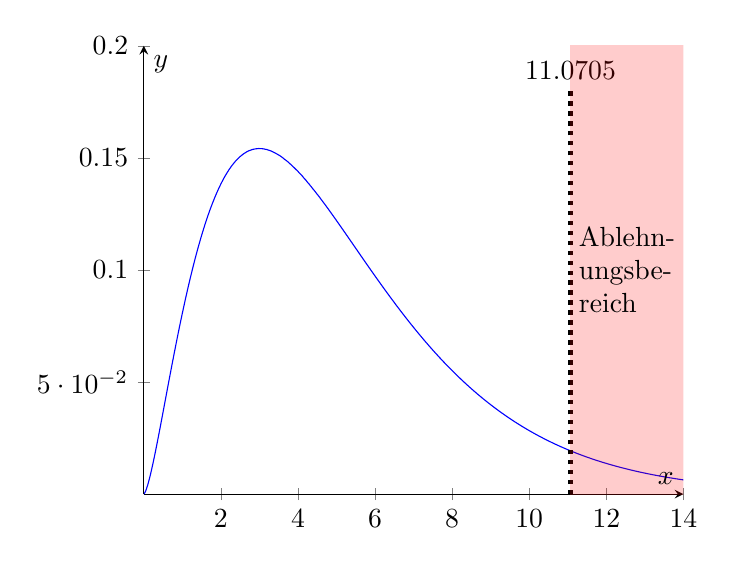
\begin{tikzpicture}
				\begin{axis}[
					xmin=0, xmax=14, xlabel=$x$,
					ymin=0, ymax=0.20, ylabel=$y$,
					samples=400,
					axis x line=middle,
					axis y line=middle,
					domain=0:14,
					]
					\addplot[mark=none,smooth,blue] {(exp(-0.5*x) * x^1.5)/(3*sqrt(2*pi))};
					
					\draw[dotted,ultra thick] (axis cs: 11.0705,0) to (axis cs: 11.0705,0.18) node[above] {11.0705};
					\draw[red,fill=red,opacity=0.2] (axis cs: 11.0705,0) rectangle (axis cs: 14,0.2) node[pos=0.5,opacity=1,black,align=left] {Ablehn-\\ungsbe-\\reich};
					
				\end{axis}
			\end{tikzpicture}
		\end{center}
		Fisher-Verteilung mit $n=2$, $m=6$, $\alpha=0.05$
		\begin{center}
			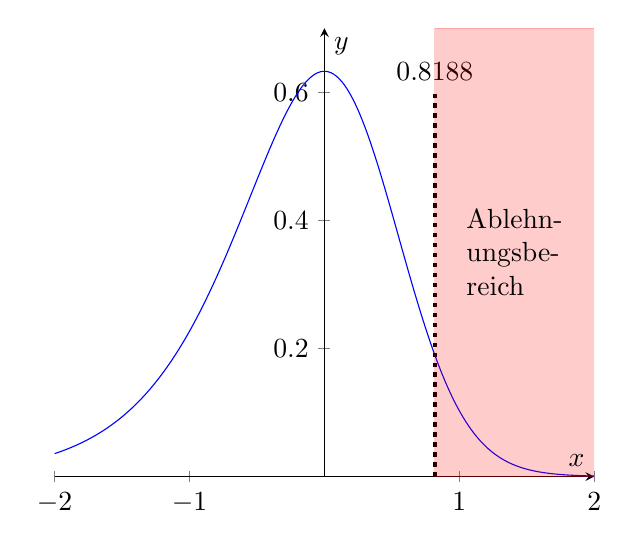
\begin{tikzpicture}
				\begin{axis}[
					xmin=-2, xmax=2, xlabel=$x$,
					ymin=0, ymax=0.7, ylabel=$y$,
					samples=400,
					axis x line=middle,
					axis y line=middle,
					domain=-4:4,
					]
					\addplot[mark=none,smooth,blue] {(2592*exp(2*x))/((2*exp(2*x) + 6)^4)};
					
					\draw[dotted,ultra thick] (axis cs: 0.8188,0) to (axis cs: 0.8188,0.6) node[above] {0.8188};
					\draw[red,fill=red,opacity=0.2] (axis cs: 0.8188,0) rectangle (axis cs: 2,0.7) node[pos=0.5,opacity=1,black,align=left] {Ablehn-\\ungsbe-\\reich};
					
				\end{axis}
			\end{tikzpicture}
		\end{center}
		\item Ablehnung von $H_0$. Im Ablehnungsbereich ist die Wahrscheinlichkeit, dass die gemessenen Daten zu $H_0$ passen, kleiner als $\alpha$.
		\item keine Ablehnung von $H_0$. Man kann sich nicht sicher sein, da eine Stichprobe nicht die Grundgesamtheit allumfänglich beschreibt. Man kann sich aber zu einem gewissen Prozentsatz sicher sein, dass die Entscheidung richtig ist $\to$ Fehler 1. und 2. Art
		\item \textit{Nicht abgelehnt} ist nicht das selbe wie \textit{Angenommen}. Insbesondere spielt beim Testen auch die Stichprobengröße eine Rolle, beim Quotienten nicht.
	\end{enumerate}

	\section*{Aufgabe 2}
	\textbf{Betrag von $t$:} Die $t$-Verteilung ist symmetrisch, es reicht also sich eine Seite (in dem Fall die rechte Seite) anzuschauen. Man muss aber bedenken, dass es beide Seiten zu betrachten gilt, deswegen $\frac{\alpha}{2}$. \\
	\textbf{Warum $1-\frac{\alpha}{2}$?} Man kann beim Testen nur sagen ob $H_0$ abgelehnt wird oder nicht, nicht ob es angenommen wird. Man betrachtet also den Ablehnungsbereich.

	\section*{Aufgabe 3}
	Wir benutzen folgendes Lemma:
	\begin{lem}
		Für Zufallsvariablen $X$, $Y$ und $Z$ gilt:
		\begin{align}
			r(X,Y) \cdot r(Y,Z) = r(X,Z) \notag
		\end{align}
	\end{lem}
	\begin{proof}
		Wir berechnen $r(X,Y) \cdot r(Y,Z)$:
		\begin{align}
			r(X,Y) \cdot r(Y,Z) &= \frac{s(X,Y) \cdot s(Y,Z)}{\sqrt{s^2(X)} \cdot \sqrt{s^2(Y)} \cdot \sqrt{s^2(Y)} \cdot \sqrt{s^2(Z)}} \notag \\
			&=\frac{\frac{1}{n-1}\left(\sum_i (x_i-\bar{x})(y_i-\bar{y}) \cdot\sum_i (y_i-\bar{y})(z_i-\bar{z})\right)}{\sqrt{s^2(X)}\sqrt{s^2(Z)}\cdot\frac{1}{n-1}\sum_i (y_i-\bar{y})^2} \notag \\
			&= \frac{\frac{1}{n-1}\left((x_1-\bar{x})(y_1-\bar{y})^2(z_1-\bar{z}) + \dots\right)}{\sqrt{s^2(X)}\sqrt{s^2(Z)}\cdot\frac{1}{n-1}\sum_i (y_i-\bar{y})^2} \notag \\
			&= \frac{s(X,Z)}{\sqrt{s^2(X)}\sqrt{s^2(Z)}} \notag \\
			&= r(X,Z) \notag
		\end{align}
	\end{proof}
	Dann gilt für die Korrelation zwischen Alter und Ausgaben $r(X_1,X_3) = r(X_1,X_2)\cdot r(X_2,X_3) = 0,9816 \cdot 0,9997 = 0,9813$.

	\section*{Aufgabe 4}
	Sei $X\sim U(-1,1)$ und $Y=X^2$. Dann gilt
	\begin{align}
		\Cov(X,Y) = \Cov(X,X^2) = \E(X^3) - \E(X)\E(X^2) = 0-0=0 \notag
	\end{align}
	Also sind $X$ und $Y$ unkorreliert, aber offensichtlich nicht unabhängig.
	
\end{document}